\documentclass[11pt]{article}
\usepackage[hmargin=1in,vmargin=1in]{geometry}
\usepackage{xcolor}
\usepackage{amsmath,amssymb,amsfonts,url,sectsty,framed,tcolorbox,framed}
\usepackage{nicematrix}
\setcounter{MaxMatrixCols}{16}
\usepackage{tikz}
\usepackage{hyperref}
\usetikzlibrary{decorations.pathreplacing}
\newcommand{\pf}{{\bf Proof: }}
\newtheorem{theorem}{Theorem}
\newtheorem{lemma}{Lemma}
\newtheorem{proposition}{Proposition}
\newtheorem{definition}{Definition}
\newtheorem{remark}{Remark}
\newcommand{\qed}{\hfill \rule{2mm}{2mm}}


\begin{document}
%%%%%%%%%%%%%%%%%%%%%%%%%%%%%%%%%%%%%%%%%%%%%%%%%%%%%%%%%%%%%%%%%%%%%
\noindent
\rule{\textwidth}{1pt}
\begin{center}
{\bf [CS304] Introduction to Cryptography and Network Security}
\end{center}
Course Instructor: Dr. Dibyendu Roy \hfill Winter 2022-2023\\
Scribed by: Chitranshi Srivastava (202051055) \hfill Lecture 10 (Week 6)
\\
\rule{\textwidth}{1pt}
%%%%%%%%%%%%%%%%%%%%%%%%%%%%%%%%%%%%%%%%%%%%%%%%%%%%%%%%%%%
%write here

In previous week, we have studied the mathematics required for understanding the AES algorithm - Generators, Subgroup, Lagrange's Theorem, Ring, Field and Field Extension, Polynomial Ring, Irreducible Polynomials and Primitivie Polynomials.

\section{Advanced Encryption Standard (AES)}

When the design of DES was made public, it was immediately broken. After that, NIST called for a competition known as Advanced Encryption Standard. There were a lot of cryptographers around the world who submitted their designs along with the implementation. One of the submission in the competition was $\emph{Rijndael}$. It was developed by two Belgian cryptographers, Joan Daemen and Vincent Rijmen. AES is unbreakable till date.\\

Advanced encryption Standard is an iterated block cipher and is based on Substitution Permutation Network(SPN). There are three different variants of AES:
\begin{enumerate}
    \item AES-128 
    \begin{itemize}
        \item Block Size 128-bit
        \item Number of Rounds = 10
        \item Secret Key Size 128-bit
    \end{itemize}    
    \item AES-192
    \begin{itemize}
        \item Block Size 128-bit
        \item Number of Rounds = 12
        \item Secret Key Size 192-bit
    \end{itemize}    
    \item AES-256 
    \begin{itemize}
        \item Block Size 128-bit
        \item Number of Rounds = 14
        \item Secret Key Size 256-bit
    \end{itemize}    
\end{enumerate}

\section{AES 128}

\begin{center}
    \tikzset{every picture/.style={line width=0.75pt}}
    
    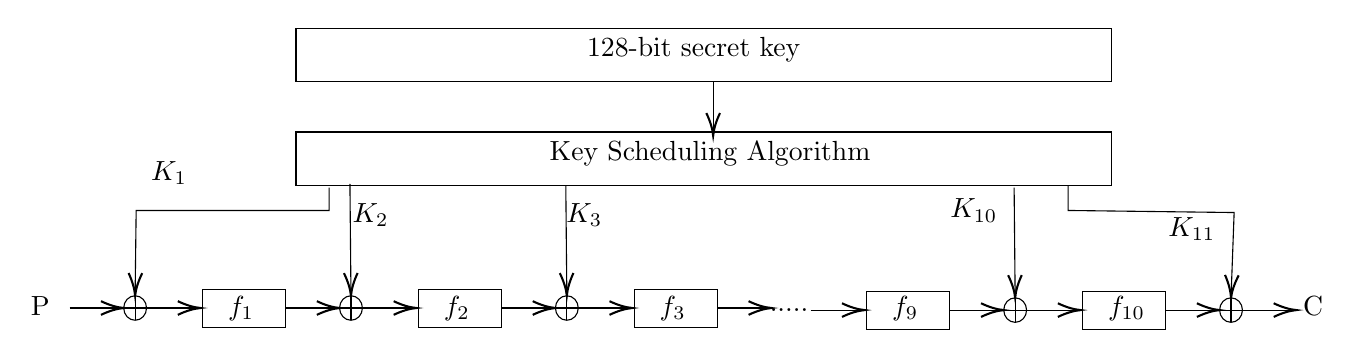
\begin{tikzpicture}[x=0.75pt,y=0.75pt,yscale=-1,xscale=1]
        \draw   (146,38) -- (539,38) -- (539,63.8) -- (146,63.8) -- cycle ;
        \draw    (347,63.8) -- (347,87.8) ;
        \draw [shift={(347,89.8)}, rotate = 270] [color={rgb, 255:red, 0; green, 0; blue, 0 }  ][line width=0.75]    (10.93,-3.29) .. controls (6.95,-1.4) and (3.31,-0.3) .. (0,0) .. controls (3.31,0.3) and (6.95,1.4) .. (10.93,3.29)   ; 
        \draw   (146,88) -- (539,88) -- (539,113.8) -- (146,113.8) -- cycle ;
        \draw    (37,172.8) -- (61,172.8) ;
        \draw [shift={(63,172.8)}, rotate = 180] [color={rgb, 255:red, 0; green, 0; blue, 0 }  ][line width=0.75]    (10.93,-3.29) .. controls (6.95,-1.4) and (3.31,-0.3) .. (0,0) .. controls (3.31,0.3) and (6.95,1.4) .. (10.93,3.29)   ;
        \draw   (63,172.8) .. controls (63,169.54) and (65.46,166.9) .. (68.5,166.9) .. controls (71.54,166.9) and (74,169.54) .. (74,172.8) .. controls (74,176.06) and (71.54,178.7) .. (68.5,178.7) .. controls (65.46,178.7) and (63,176.06) .. (63,172.8) -- cycle ; \draw   (63,172.8) -- (74,172.8) ; \draw   (68.5,166.9) -- (68.5,178.7) ;
        \draw    (74,172.8) -- (98,172.8) ;
        \draw [shift={(100,172.8)}, rotate = 180] [color={rgb, 255:red, 0; green, 0; blue, 0 }  ][line width=0.75]    (10.93,-3.29) .. controls (6.95,-1.4) and (3.31,-0.3) .. (0,0) .. controls (3.31,0.3) and (6.95,1.4) .. (10.93,3.29)   ;
        \draw   (101,163.8) -- (141,163.8) -- (141,182) -- (101,182) -- cycle ;
        \draw    (141,172.8) -- (165,172.8) ;
        \draw [shift={(167,172.8)}, rotate = 180] [color={rgb, 255:red, 0; green, 0; blue, 0 }  ][line width=0.75]    (10.93,-3.29) .. controls (6.95,-1.4) and (3.31,-0.3) .. (0,0) .. controls (3.31,0.3) and (6.95,1.4) .. (10.93,3.29)   ;
        \draw   (167,172.8) .. controls (167,169.54) and (169.46,166.9) .. (172.5,166.9) .. controls (175.54,166.9) and (178,169.54) .. (178,172.8) .. controls (178,176.06) and (175.54,178.7) .. (172.5,178.7) .. controls (169.46,178.7) and (167,176.06) .. (167,172.8) -- cycle ; \draw   (167,172.8) -- (178,172.8) ; \draw   (172.5,166.9) -- (172.5,178.7) ;
        \draw    (178,172.8) -- (202,172.8) ;
        \draw [shift={(204,172.8)}, rotate = 180] [color={rgb, 255:red, 0; green, 0; blue, 0 }  ][line width=0.75]    (10.93,-3.29) .. controls (6.95,-1.4) and (3.31,-0.3) .. (0,0) .. controls (3.31,0.3) and (6.95,1.4) .. (10.93,3.29)   ; 
        \draw   (205,163.8) -- (245,163.8) -- (245,182) -- (205,182) -- cycle ; 
        \draw    (245,172.8) -- (269,172.8) ;
        \draw [shift={(271,172.8)}, rotate = 180] [color={rgb, 255:red, 0; green, 0; blue, 0 }  ][line width=0.75]    (10.93,-3.29) .. controls (6.95,-1.4) and (3.31,-0.3) .. (0,0) .. controls (3.31,0.3) and (6.95,1.4) .. (10.93,3.29)   ; 
        \draw   (271,172.8) .. controls (271,169.54) and (273.46,166.9) .. (276.5,166.9) .. controls (279.54,166.9) and (282,169.54) .. (282,172.8) .. controls (282,176.06) and (279.54,178.7) .. (276.5,178.7) .. controls (273.46,178.7) and (271,176.06) .. (271,172.8) -- cycle ; \draw   (271,172.8) -- (282,172.8) ; \draw   (276.5,166.9) -- (276.5,178.7) ;
        \draw    (282,172.8) -- (306,172.8) ;
        \draw [shift={(308,172.8)}, rotate = 180] [color={rgb, 255:red, 0; green, 0; blue, 0 }  ][line width=0.75]    (10.93,-3.29) .. controls (6.95,-1.4) and (3.31,-0.3) .. (0,0) .. controls (3.31,0.3) and (6.95,1.4) .. (10.93,3.29)   ;
        \draw   (309,163.8) -- (349,163.8) -- (349,182) -- (309,182) -- cycle ;
        \draw    (349,172.8) -- (373,172.8) ;
        \draw [shift={(375,172.8)}, rotate = 180] [color={rgb, 255:red, 0; green, 0; blue, 0 }  ][line width=0.75]    (10.93,-3.29) .. controls (6.95,-1.4) and (3.31,-0.3) .. (0,0) .. controls (3.31,0.3) and (6.95,1.4) .. (10.93,3.29)   ;
        \draw    (394,173.8) -- (418,173.8) ;
        \draw [shift={(420,173.8)}, rotate = 180] [color={rgb, 255:red, 0; green, 0; blue, 0 }  ][line width=0.75]    (10.93,-3.29) .. controls (6.95,-1.4) and (3.31,-0.3) .. (0,0) .. controls (3.31,0.3) and (6.95,1.4) .. (10.93,3.29)   ;
        \draw   (421,164.8) -- (461,164.8) -- (461,183) -- (421,183) -- cycle ;
        \draw    (461,173.8) -- (485,173.8) ;
        \draw [shift={(487,173.8)}, rotate = 180] [color={rgb, 255:red, 0; green, 0; blue, 0 }  ][line width=0.75]    (10.93,-3.29) .. controls (6.95,-1.4) and (3.31,-0.3) .. (0,0) .. controls (3.31,0.3) and (6.95,1.4) .. (10.93,3.29)   ;
        \draw   (487,173.8) .. controls (487,170.54) and (489.46,167.9) .. (492.5,167.9) .. controls (495.54,167.9) and (498,170.54) .. (498,173.8) .. controls (498,177.06) and (495.54,179.7) .. (492.5,179.7) .. controls (489.46,179.7) and (487,177.06) .. (487,173.8) -- cycle ; \draw   (487,173.8) -- (498,173.8) ; \draw   (492.5,167.9) -- (492.5,179.7) ;
        \draw    (498,173.8) -- (522,173.8) ;
        \draw [shift={(524,173.8)}, rotate = 180] [color={rgb, 255:red, 0; green, 0; blue, 0 }  ][line width=0.75]    (10.93,-3.29) .. controls (6.95,-1.4) and (3.31,-0.3) .. (0,0) .. controls (3.31,0.3) and (6.95,1.4) .. (10.93,3.29)   ;
        \draw   (525,164.8) -- (565,164.8) -- (565,183) -- (525,183) -- cycle ;
        \draw    (565,173.8) -- (589,173.8) ;
        \draw [shift={(591,173.8)}, rotate = 180] [color={rgb, 255:red, 0; green, 0; blue, 0 }  ][line width=0.75]    (10.93,-3.29) .. controls (6.95,-1.4) and (3.31,-0.3) .. (0,0) .. controls (3.31,0.3) and (6.95,1.4) .. (10.93,3.29)   ;
        \draw   (591,173.8) .. controls (591,170.54) and (593.46,167.9) .. (596.5,167.9) .. controls (599.54,167.9) and (602,170.54) .. (602,173.8) .. controls (602,177.06) and (599.54,179.7) .. (596.5,179.7) .. controls (593.46,179.7) and (591,177.06) .. (591,173.8) -- cycle ; \draw   (591,173.8) -- (602,173.8) ; \draw   (596.5,167.9) -- (596.5,179.7) ; 
        \draw    (602,173.8) -- (626,173.8) ;
        \draw [shift={(628,173.8)}, rotate = 180] [color={rgb, 255:red, 0; green, 0; blue, 0 }  ][line width=0.75]    (10.93,-3.29) .. controls (6.95,-1.4) and (3.31,-0.3) .. (0,0) .. controls (3.31,0.3) and (6.95,1.4) .. (10.93,3.29)   ;
        \draw    (162,114.8) -- (162,125.8) -- (69,125.8) -- (68.52,164.9) ;
        \draw [shift={(68.5,166.9)}, rotate = 270.7] [color={rgb, 255:red, 0; green, 0; blue, 0 }  ][line width=0.75]    (10.93,-3.29) .. controls (6.95,-1.4) and (3.31,-0.3) .. (0,0) .. controls (3.31,0.3) and (6.95,1.4) .. (10.93,3.29)   ;
        \draw    (172,113) -- (172.48,164.9) ;
        \draw [shift={(172.5,166.9)}, rotate = 269.47] [color={rgb, 255:red, 0; green, 0; blue, 0 }  ][line width=0.75]    (10.93,-3.29) .. controls (6.95,-1.4) and (3.31,-0.3) .. (0,0) .. controls (3.31,0.3) and (6.95,1.4) .. (10.93,3.29)   ;
        \draw    (276,113.8) -- (276.48,164.9) ;
        \draw [shift={(276.5,166.9)}, rotate = 269.46] [color={rgb, 255:red, 0; green, 0; blue, 0 }  ][line width=0.75]    (10.93,-3.29) .. controls (6.95,-1.4) and (3.31,-0.3) .. (0,0) .. controls (3.31,0.3) and (6.95,1.4) .. (10.93,3.29)   ;
        \draw    (492,114.8) -- (492.48,165.9) ;
        \draw [shift={(492.5,167.9)}, rotate = 269.46] [color={rgb, 255:red, 0; green, 0; blue, 0 }  ][line width=0.75]    (10.93,-3.29) .. controls (6.95,-1.4) and (3.31,-0.3) .. (0,0) .. controls (3.31,0.3) and (6.95,1.4) .. (10.93,3.29)   ;
        \draw    (518,113.8) -- (518,125.8) -- (598,126.8) -- (596.57,165.9) ;
        \draw [shift={(596.5,167.9)}, rotate = 272.09] [color={rgb, 255:red, 0; green, 0; blue, 0 }  ][line width=0.75]    (10.93,-3.29) .. controls (6.95,-1.4) and (3.31,-0.3) .. (0,0) .. controls (3.31,0.3) and (6.95,1.4) .. (10.93,3.29)   ;
        
        \draw (285,41) node [anchor=north west][inner sep=0.75pt]   [align=left] {128-bit secret key};
        \draw (267,91) node [anchor=north west][inner sep=0.75pt]   [align=left] {Key Scheduling Algorithm};
        \draw (17,166) node [anchor=north west][inner sep=0.75pt]   [align=left] {P};
        \draw (112,166) node [anchor=north west][inner sep=0.75pt]   [align=left] {$f_1$};
        \draw (216,166) node [anchor=north west][inner sep=0.75pt]   [align=left] {$f_2$};
        \draw (320,166) node [anchor=north west][inner sep=0.75pt]   [align=left] {$f_3$};
        \draw (373,172) node [anchor=north west][inner sep=0.75pt]   [align=left] {.....};
        \draw (432,166) node [anchor=north west][inner sep=0.75pt]   [align=left] {$f_9$};
        \draw (536,166) node [anchor=north west][inner sep=0.75pt]   [align=left] {$f_{10}$};
        \draw (630,166) node [anchor=north west][inner sep=0.75pt]   [align=left] {C};
        \draw (75,101) node [anchor=north west][inner sep=0.75pt]   [align=left] {$K_1$};
        \draw (172,121) node [anchor=north west][inner sep=0.75pt]   [align=left] {$K_2$};
        \draw (275,121) node [anchor=north west][inner sep=0.75pt]   [align=left] {$K_3$};
        \draw (460,119) node [anchor=north west][inner sep=0.75pt]   [align=left] {$K_{10}$};
        \draw (565,128) node [anchor=north west][inner sep=0.75pt]   [align=left] {$K_{11}$};
    \end{tikzpicture}
\end{center}
The diagram above depicts the encryption process. \\
The Key Scheduling Algorithm takes 128-bit key as input and generates 11 round keys of 128-bit each. The plaintext P is xored with $K_1$(first round key). This value is input to $f_1$(first round function) which produces 128-bit output. This output is cored with $K_2$(second round key) and the output is passed to $f_2$(second round function). Again, $f_2$ produces 128-bit output and this will continue till $f_{10}$. Finally, output of $f_{10}$ will be xored with $K_{11}$(last round key) and this output will be our ciphertext.\\

\vspace{3mm}
Given the ciphertext, decryption process will begin with xoring the ciphertext with $K_{11}$(last round key) and this output will be input to inverse of $f_{10}$ function. Inverse of $f_{10}$ function will generate a 128-bit output which will be xored with $K_{10}$, and output will be passed to inverse of $f_9$ function, and so on it will be continued till inverse of $f_1$ function. The output will be xored with $K_1$(first round key) to get the plaintext.\\
\newline
\textbf{Note:} The decryption process described above clearly states that the round functions $f_1, f_2,..., f_{10}$ must be invertible. Hence, this structure is different from Feistel Network where the invertibility of round functions does not matter. \\
Now, we need to understand the following things:
\begin{itemize}
    \item Round Functions
    \item Key Scheduling Algorithm
\end{itemize}

\subsection{Round Functions of AES-128}
The round functions $f_1, f_2,..., f_{10}$ are a mapping from 128-bit to 128-bit.
\begin{center}
    $f_i : \{0, 1\}^{128} \rightarrow \{0, 1\}^{128}$ $\forall$ $ 1 \leq i \leq 10$
\end{center}
The first 9 round functions $f_1, f_2,..., f_9$ are same and are different from the last round function $f_{10}$. This is true for other variants of AES too. The last round function is different from the other round functions. All the round functions are same except the last one.\\
\newline
The first 9 round functions $f_1, f_2,..., f_9$ are based on the following three functions:
\begin{itemize}
    \item Subbytes
    \item Shift Rows
    \item Mix Columns
\end{itemize}
And for the last round function, we have the following steps:
\begin{itemize}
    \item Subbytes
    \item Shift Rows
\end{itemize}
For the first 9 round functions:
\begin{center}
    $f_i(X) = MixColumns(ShiftRows(Subbytes(X)))$ $\forall$ $1 \leq i \leq 9$
\end{center}
However, the last round function $f_{10}$ is based on subbytes and shift rows only. Therefore,
\begin{center}
    $f_{10}(X) = ShiftRows(Subbytes(X))$
\end{center}

Each Subbyte, Shift Rows and Mix Columns is a bijection from 128-bit to 128-bit. This means each of them has existing inverse. Therefore, given $y = f_i(X)$, to get $X$, apply inverse of mix columns, then apply inverse of Shift Rows and then apply inverse of Subbytes.\\
\newline
For the first 9 rounds $f_1, f_2,..., f_9$:
\begin{center}
    \tikzset{every picture/.style={line width=0.75pt}} 
    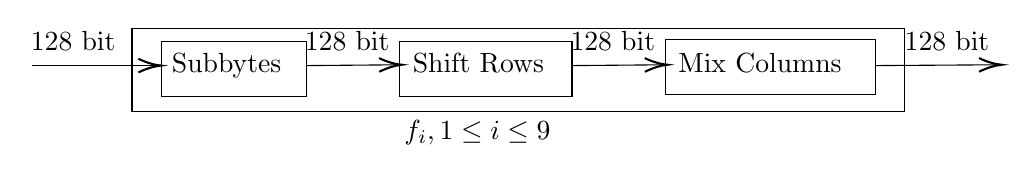
\begin{tikzpicture}[x=0.75pt,y=0.75pt,yscale=-1,xscale=1]
        \draw   (139,298.6) -- (511,298.6) -- (511,338.6) -- (139,338.6) -- cycle ;
        \draw   (153,305.2) -- (223,305.2) -- (223,331.6) -- (153,331.6) -- cycle ;
        \draw   (268,305.2) -- (351,305.2) -- (351,331.6) -- (268,331.6) -- cycle ;
        \draw   (396,304.2) -- (497,304.2) -- (497,330.6) -- (396,330.6) -- cycle ;
        \draw    (223,316.6) -- (267,316.22) ;
        \draw [shift={(269,316.2)}, rotate = 179.5] [color={rgb, 255:red, 0; green, 0; blue, 0 }  ][line width=0.75]    (10.93,-3.29) .. controls (6.95,-1.4) and (3.31,-0.3) .. (0,0) .. controls (3.31,0.3) and (6.95,1.4) .. (10.93,3.29)   ;
        \draw    (351,316.6) -- (395,316.22) ;
        \draw [shift={(397,316.2)}, rotate = 179.5] [color={rgb, 255:red, 0; green, 0; blue, 0 }  ][line width=0.75]    (10.93,-3.29) .. controls (6.95,-1.4) and (3.31,-0.3) .. (0,0) .. controls (3.31,0.3) and (6.95,1.4) .. (10.93,3.29)   ;
        \draw    (91,316.6) -- (151,316.6) ;
        \draw [shift={(153,316.6)}, rotate = 180] [color={rgb, 255:red, 0; green, 0; blue, 0 }  ][line width=0.75]    (10.93,-3.29) .. controls (6.95,-1.4) and (3.31,-0.3) .. (0,0) .. controls (3.31,0.3) and (6.95,1.4) .. (10.93,3.29)   ;
        \draw    (497,316.6) -- (556,316.21) ;
        \draw [shift={(558,316.2)}, rotate = 179.62] [color={rgb, 255:red, 0; green, 0; blue, 0 }  ][line width=0.75]    (10.93,-3.29) .. controls (6.95,-1.4) and (3.31,-0.3) .. (0,0) .. controls (3.31,0.3) and (6.95,1.4) .. (10.93,3.29)   ;
        
        \draw (157,309.2) node [anchor=north west][inner sep=0.75pt]   [align=left] {Subbytes};
        \draw (273,309.2) node [anchor=north west][inner sep=0.75pt]   [align=left] {Shift Rows};
        \draw (401,309.2) node [anchor=north west][inner sep=0.75pt]   [align=left] {Mix Columns};
        \draw (221,298.6) node [anchor=north west][inner sep=0.75pt]   [align=left] {128 bit};
        \draw (349,298.6) node [anchor=north west][inner sep=0.75pt]   [align=left] {128 bit};
        \draw (89,298.6) node [anchor=north west][inner sep=0.75pt]   [align=left] {128 bit};
        \draw (510,298.6) node [anchor=north west][inner sep=0.75pt]   [align=left] {128 bit};
        \draw (269,341.6) node [anchor=north west][inner sep=0.75pt]   [align=left] {$f_i, 1 \leq i \leq 9$};
    \end{tikzpicture}
\end{center}

For the last round function $f_{10}$:
\begin{center}
    \tikzset{every picture/.style={line width=0.75pt}} 

    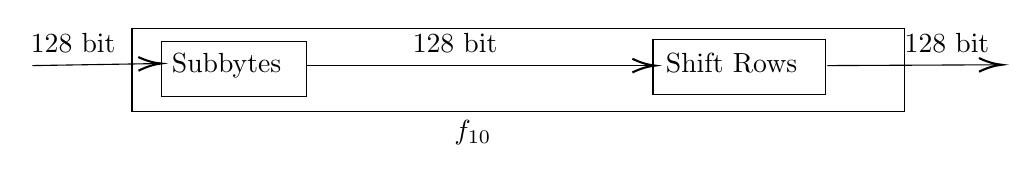
\begin{tikzpicture}[x=0.75pt,y=0.75pt,yscale=-1,xscale=1] 
        \draw   (146,426.6) -- (518,426.6) -- (518,466.6) -- (146,466.6) -- cycle ;
        \draw   (160,433.2) -- (230,433.2) -- (230,459.6) -- (160,459.6) -- cycle ;
        \draw   (397,432.2) -- (480,432.2) -- (480,458.6) -- (397,458.6) -- cycle ;
        \draw    (230,444.6) -- (396,444.6) ;
        \draw [shift={(398,444.6)}, rotate = 180] [color={rgb, 255:red, 0; green, 0; blue, 0 }  ][line width=0.75]    (10.93,-3.29) .. controls (6.95,-1.4) and (3.31,-0.3) .. (0,0) .. controls (3.31,0.3) and (6.95,1.4) .. (10.93,3.29)   ; 
        \draw    (98,444.6) -- (158,443.63) ;
        \draw [shift={(160,443.6)}, rotate = 179.08] [color={rgb, 255:red, 0; green, 0; blue, 0 }  ][line width=0.75]    (10.93,-3.29) .. controls (6.95,-1.4) and (3.31,-0.3) .. (0,0) .. controls (3.31,0.3) and (6.95,1.4) .. (10.93,3.29)   ;
        \draw    (481,444.6) -- (563,444.21) ;
        \draw [shift={(565,444.2)}, rotate = 179.73] [color={rgb, 255:red, 0; green, 0; blue, 0 }  ][line width=0.75]    (10.93,-3.29) .. controls (6.95,-1.4) and (3.31,-0.3) .. (0,0) .. controls (3.31,0.3) and (6.95,1.4) .. (10.93,3.29)   ;
        
        \draw (164,437.2) node [anchor=north west][inner sep=0.75pt]   [align=left] {Subbytes};
        \draw (402,437.2) node [anchor=north west][inner sep=0.75pt]   [align=left] {Shift Rows};
        \draw (280,427.6) node [anchor=north west][inner sep=0.75pt]   [align=left] {128 bit};
        \draw (96,427.6) node [anchor=north west][inner sep=0.75pt]   [align=left] {128 bit};
        \draw (517,427.6) node [anchor=north west][inner sep=0.75pt]   [align=left] {128 bit};
        \draw (300,469.6) node [anchor=north west][inner sep=0.75pt]   [align=left] {$f_{10}$};
    \end{tikzpicture}
\end{center}

\subsubsection{Subbytes}
Subbytes is a bijective mapping from 128-bit to 128-bit.
\begin{center}
    Subbytes: $\{0, 1\}^{128} \rightarrow \{0, 1\}^{128}$
\end{center}
The input S to subbytes function is a 128-bit binary input. A $4 \times 4$ matrix can be constructed from the input in the following way:
\begin{center}
    $S \rightarrow  
        \begin{bmatrix}
        S_{00} & S_{01} & S_{02} & S_{03}\\
        S_{10} & S_{11} & S_{12} & S_{13}\\
        S_{20} & S_{21} & S_{22} & S_{23}\\
        S_{30} & S_{31} & S_{32} & S_{33}\\
        \end{bmatrix}$
\end{center}
where $S_{ij}$ is a byte (8-bits). Consider the 128-bit plaintext of 128-bit. The plaintext again can be written as a $4 \times 4$ matrix in the following way. Keep in mind, the ordering of the plaintext bytes.
\begin{center}
    $P = P_0P_1P_2....P_{15}$, length of each $P_i$ is 8-bit\\
    \vspace{1mm}
    $P \rightarrow  
        \begin{bmatrix}
        P_0 & P_4 & P_8 & P_{12}\\
        P_1 & P_5 & P_9 & P_{13}\\
        P_2 & P_6 & P_{10} & P_{14}\\
        P_3 & P_7 & P_{11} & P_{15}\\
        \end{bmatrix}$
\end{center}
Similarly, the first round key $K_1$ can also be written as a matrix.
\begin{center}
    $K_1 = K_0K_1K_2....K_{15}$, length of each $K_i$ is 8-bit\\
    \vspace{1mm}
    $K_1 \rightarrow  
        \begin{bmatrix}
        K_0 & K_4 & K_8 & K_{12}\\
        K_1 & K_5 & K_9 & K_{13}\\
        K_2 & K_6 & K_{10} & K_{14}\\
        K_3 & K_7 & K_{11} & K_{15}\\
        \end{bmatrix}$
\end{center}
For AES-128, we first xor the plaintext with the first round key $K_1$. The output is then passed to first round function, wherein, it is first passed to subbytes function.
\begin{center}
    $S = (S_{ij})_{4 \times 4} = P \oplus K_1$
\end{center}
The output after the subbyte function is performed on S is $S'$.
\begin{center}
    $S' = Subbytes(S)$
\end{center}

Now, let us look at how the subbyte function works. The following steps are followed in order to get the output from subbyte function.
\begin{enumerate}
    \item Declare a constant C = $C_7C_6C_5C_4C_3C_2C_1C_0 = (01100011) = (63)_{16}$
    \item There is a substitution box $\mathbb{S}$ from 8-bit to 8-bit. This $\mathbb{S}$ box is applied to every element of S matrix, i.e, $S_{ij}$. Also, $\mathbb{S}(0) = 0$ is always true.
    \item Now, let's say $\mathbb{S}(S_{ij}) = m_7m_6m_5m_4m_3m_2m_1m_0$.
    \item For i = 0 to i = 7, compute $b_i$ as:
    \begin{center}
        $b_i = (m_i + m_{(i+4)\%8} + m_{(i+5)\%8} + m_{(i+6)\%8} + m_{(i+7)\%8} + C_i) \% 2$
    \end{center}
    \item Therefore, the output is $b_7b_6b_5b_4b_3b_2b_1b_0$.
    \item $S'_{ij} = (b_7b_6b_5b_4b_3b_2b_1b_0)$
\end{enumerate}
Hence, $S'_{ij}$ is computed for each $S_{ij}$ and the output matrix is the output of subbyte function.
\begin{center}
    $
    \begin{bmatrix}
        S_{00} & S_{01} & S_{02} & S_{03}\\
        S_{10} & S_{11} & S_{12} & S_{13}\\
        S_{20} & S_{21} & S_{22} & S_{23}\\
        S_{30} & S_{31} & S_{32} & S_{33}\\
    \end{bmatrix}
    \xrightarrow{Subbyte}
    \begin{bmatrix}
        S'_{00} & S'_{01} & S'_{02} & S'_{03}\\
        S'_{10} & S'_{11} & S'_{12} & S'_{13}\\
        S'_{20} & S'_{21} & S'_{22} & S'_{23}\\
        S'_{30} & S'_{31} & S'_{32} & S'_{33}\\
    \end{bmatrix}
    $
\end{center}

Now, we will discuss the substitution box $\mathbb{S}$ that takes 8-bit input and produces 8-bit output.
\begin{center}
    $\mathbb{S}: \{0, 1\}^8 \rightarrow \{0, 1\}^8$ and $\mathbb{S}(0) = 0$
\end{center}
Let's say input X is given to this $\mathbb{S}$ box and $X \neq 0$. We need to find $Y = \mathbb{S}(X)$.
\begin{center}
    $X = a_7a_6a_5a_4a_3a_2a_1a_0$, where $a_i \in \{0, 1\}$
\end{center}
We can construct a polynomial $P(x)$ using the bits of X as coefficients.
\begin{center}
    $P(x) = a_0 + a_1 \cdot x + a_2 \cdot x^2 +.....+ a_7 \cdot x^7$
\end{center}
Clearly, degree of $P(x) \leq 7$. Also, $P(x) \in F_2[x]$. Moreover, since $X \neq 0 \implies P(x) \neq 0$. Another polynomial $g(x) = x^8 + x^4 + x^3 + x + 1$ is fixed for AES. $g(x)$ is a primitive polynomial.\\
\newline
Since, $g(x)$ is primitive, $(F_2[x]/\langle g(x) \rangle, +, *)$ is a field where $+$ is addition modulo $g(x)$ and $*$ is multiplication modulo $g(x)$. All the polynomials in the above field will have at most degree 7. Therefore, $P(x)$ belongs to above field. Also, since $\langle g(x) \rangle$ is primitive, we can find multiplicative inverse of any polynomial in $(F_2[x]/\langle g(x) \rangle)$. Therefore, we will find the multiplicative inverse of $P(x)$ under modulo $g(x)$. Let's say the multiplicative inverse of $P(x)$ under modulo $g(x)$ be $q(x)$. Therefore, 
\begin{center}
    $P(x)\cdot q(x) \equiv 1 mod $ $g(x)$\\
    \vspace{1mm}
    $P(x) \cdot q(x) \equiv 1 mod (x^8 + x^4 + x^3 + x + 1)$\\
    \vspace{1mm}
    $P(x)\cdot q(x) - 1 = h(x) \cdot (x^8 + x^4 + x^3 + x + 1)$\\
    \vspace{1mm}
    $1 = P(x) \cdot q(x) + h(x) \cdot (x^8 + x^4 + x^3 + x + 1)$
\end{center}
Therefore, we can find the $q(x)$ with the help of Extended Euclidean Algorithm. Also, $q(x)$ will be a polynomial of degree at most 7.
\begin{center}
    $q(x) = r_0 + r_1\cdot x+ r_2 \cdot x^2 +.....+ r_7 \cdot x^7$, where $r_i \in \{0, 1\}$
\end{center}
From the coefficients, we can build a 8-bit binary string as $r_7r_6r_5r_4r_3r_2r_1r_0$. This string is the output of the $\mathbb{S}$ box. Therefore,
\begin{center}
    $\mathbb{S}(X) = Y = (r_7r_6r_5r_4r_3r_2r_1r_0)$
\end{center}

\textbf{Example:} Find Subbytes(01010011).\\
\textbf{Solution:} X = 01010011, therefore $P(x) = x^6 + x^4 + x + 1$. Also, $g(x) = x^8 + x^4 + x^3 + x + 1$. Now, let's perform the Extended Euclidean Algorithm.
\begin{center}
    \tikzset{every picture/.style={line width=0.75pt}} 

    \begin{tikzpicture}[x=0.75pt,y=0.75pt,yscale=-1,xscale=1]
%uncomment if require: \path (0,529); %set diagram left start at 0, and has height of 529
        
        %Straight Lines [id:da7065959490003173] 
        \draw    (163,171.2) -- (363,171.2) ;
        %Straight Lines [id:da028549667874976592] 
        \draw    (182,230.2) -- (339,231.2) ;
        %Straight Lines [id:da899367259935002] 
        \draw    (186,283.2) -- (343,284.2) ;
        %Straight Lines [id:da4356732499452918] 
        \draw    (292,284.2) -- (449,285.2) ;
        %Straight Lines [id:da9322638753565391] 
        \draw    (304,336.2) -- (439,337.2) ;
        %Straight Lines [id:da9488931091504231] 
        \draw    (359,381.2) -- (510,381.2) ;
        %Straight Lines [id:da18220626076094226] 
        \draw    (446,441.2) -- (510,440.2) ;
        %Straight Lines [id:da7371705002655333] 
        \draw    (488,481.2) -- (528,480.2) ;
        %Straight Lines [id:da7407976464457187] 
        \draw    (489,501.2) -- (529,500.2) ;
        
        \draw (158,169) node [anchor=north west][inner sep=0.75pt]   [align=left] {{\Huge )}};
        \draw (187,178) node [anchor=north west][inner sep=0.75pt]   [align=left] {$x^8 + x^4 + x^3 + x + 1$};
        \draw (351,169) node [anchor=north west][inner sep=0.75pt]   [align=left] {{\Huge (}};
        \draw (60,177) node [anchor=north west][inner sep=0.75pt]   [align=left] {$x^6 + x^4 + x + 1$};
        \draw (359,177) node [anchor=north west][inner sep=0.75pt]   [align=left] {$x^2 + 1$};
        \draw (185,205) node [anchor=north west][inner sep=0.75pt]   [align=left] {$x^8 + x^6 + x^3 + x^2$};
        \draw (186,238) node [anchor=north west][inner sep=0.75pt]   [align=left] {$x^6 + x^4 + x^2 + x + 1$};
        \draw (185,261) node [anchor=north west][inner sep=0.75pt]   [align=left] {$x^6 + x^4 + x + 1$};
        \draw (285,282) node [anchor=north west][inner sep=0.75pt]   [align=left] {{\Huge )}};
        \draw (438,283) node [anchor=north west][inner sep=0.75pt]   [align=left] {{\Huge (}};
        \draw (267,290) node [anchor=north west][inner sep=0.75pt]   [align=left] {$x^2$};
        \draw (453,292) node [anchor=north west][inner sep=0.75pt]   [align=left] {$x^4 + x^2$};
        \draw (314,289) node [anchor=north west][inner sep=0.75pt]   [align=left] {$x^6 + x^4 + x + 1$};
        \draw (315,315) node [anchor=north west][inner sep=0.75pt]   [align=left] {$x^6$};
        \draw (358,338) node [anchor=north west][inner sep=0.75pt]   [align=left] {$x^4+ x + 1$};
        \draw (359,359) node [anchor=north west][inner sep=0.75pt]   [align=left] {$x^4$};
        \draw (399,387) node [anchor=north west][inner sep=0.75pt]   [align=left] {$x + 1$};
        \draw (433,379) node [anchor=north west][inner sep=0.75pt]   [align=left] {{\Huge )}};
        \draw (497,380) node [anchor=north west][inner sep=0.75pt]   [align=left] {{\Huge (}};
        \draw (460,387) node [anchor=north west][inner sep=0.75pt]   [align=left] {$x^2$};
        \draw (515,386) node [anchor=north west][inner sep=0.75pt]   [align=left] {$x + 1$};
        \draw (448,416) node [anchor=north west][inner sep=0.75pt]   [align=left] {$x^2 + x$};
        \draw (486,445) node [anchor=north west][inner sep=0.75pt]   [align=left] {$x$};
        \draw (486,458) node [anchor=north west][inner sep=0.75pt]   [align=left] {$x + 1$};
        \draw (508,482.7) node [anchor=north west][inner sep=0.75pt]   [align=left] {$1$};
    \end{tikzpicture}
\end{center}
Now, let's work upside down to find the multiplicative inverse. Therefore,
    $1 = q(x)\cdot P(x) = h(x) \cdot g(x)$\\
    \vspace{2mm}
    $1 = 1 \cdot x^2 + (x+1) \cdot (x+1)$\\
    \vspace{2mm}
    $1 = x^2 + (x + 1) \cdot [(x^6 + x^4 + x + 1) + x^2 \cdot (x^4 + x^2)]$\\
    \vspace{2mm}
    $1 = (x+1) \cdot (x^6 + x^4 + x + 1) + x^2 \cdot [1 + (x+1) \cdot (x^4 + x^2)]$\\
    \vspace{2mm}
    $1 = (x+1) \cdot (x^6 + x^4 + x + 1) + x^2 \cdot (x^5 + x^4 + x^3 + x^2 + 1)$\\
    \vspace{2mm}
    $1 = (x+1) \cdot (x^6 + x^4 + x + 1) + (x^5 + x^4 + x^3 + x^2 + 1) \cdot [(x^8 + x^4 + x^3 + x + 1) + (x^6 + x^4 + x + 1) \cdot (x^2 + 1)] $\\
    \vspace{2mm}
    $1 = [(x + 1) + (x^2 + 1) \cdot (x^5 + x^4 + x^3 + x^2 + 1)] \cdot P(x) + (x^5 + x^4 + x^3 + x^2 + 1) \cdot g(x)$\\
    \vspace{2mm}
    $1 = (x + 1 + x^7 + x^6 + x^5 + x^4 + x^2 + x^5 + x^4 + x^3 + x^2 + 1) \cdot P(x) + (x^5 + x^4 + x^3 + x^2 + 1) \cdot g(x)$\\
    \vspace{2mm}
    $1 = (x^7 + x^6 + x^3 + x) \cdot P(x) + (x^5 + x^4 + x^3 + x^2 + 1) \cdot g(x)$\\
Therefore, Multiplicative Inverse of P(x) is $q(x) = x^7 + x^6 + x^3 + x$. Therefore,
\begin{center}
    $\mathbb{S}(01010011) = (11001010) = m_7m_6m_5m_4m_3m_2m_1m_0$
\end{center}
Now, let's compute $b_7b_6b_5b_4b_3b_2b_1b_0$. The constant C = $c_7c_6c_5c_4c_3c_2c_1c_0 = 01100011$.
\begin{center}
    \begin{tabular}{|c|c|c|c|c|c|c|c|c|}
        \hline
         & 0 & 1 & 2 & 3 & 4 & 5 & 6 & 7 \\ \hline
        c & 1 & 1 & 0 & 0 & 0 & 1 & 1 & 0  \\ \hline
        m & 0 & 1 & 0 & 1 & 0 & 0 & 1 & 1  \\ \hline
    \end{tabular}
\end{center}
\begin{center}
    $b_0 = (0 + 0 + 0 + 1 + 1 + 1) \% 2 = 1$\\
    $b_1 = (1 + 0 + 1 + 1 + 0 + 1) \%2 = 0$\\
    $b_2 = 1, b_3 = 1, b_4 = 0$\\
    $b_5 = 1, b_6 = 1, b_7 = 1$\\
    $\therefore subbytes(01010011) = b_7b_6b_5b_4b_3b_2b_1b_0 = (11101101)$\\
    $subbytes(53) = (ED)$
\end{center}

The 8-bit to 8-bit mapping can be stores separately in a table of 256 inputs and corresponding 256 outputs with a memory of just $2^8 \times 8$ bits. Hence, this computation is not done. The value is looked up in a $16 \times 16 table$.
\begin{center}
    Input = XY\\
    Subbyte(Input) $\rightarrow$ element present in row number X and column number Y
\end{center}
The lookup table is given in the Handbook of Cryptography book and we can verify the above example using that.


\end{document}